\documentclass[10 pt,usenames,dvipsnames, oneside]{article}
\usepackage{../../../modelo-ensino-medio}



\begin{document}

\begin{center}
  \begin{minipage}[l]{3cm}

\includegraphics[width=2cm]{logo}    
\end{minipage}\hfill
\begin{minipage}[r]{.8\textwidth}
 {\Large \scshape Atividade: Construção do Histograma}  
\end{minipage}
\end{center}
\vspace{.2cm}

\ifdefined\prof
\begin{objetivos}
\item \textbf{EM13MAT406}: Construir e interpretar tabelas e gráficos de frequências com base em dados obtidos em pesquisas por amostras estatísticas, incluindo ou não o uso de softwares que interrelacionem estatística, geometria e álgebra.
\end{objetivos}

\begin{goals}
\begin{enumerate}
\item Identificar, na construção de um gráfico que represente a distribuição de frequências, a necessidade de agrupar em intervalos de classe os valores observados de uma variável quantitativa contínua.
\end{enumerate}

\tcblower

A construção do histograma será dirigida nessa atividade, mas recomenda-se fortemente o uso de recursos tecnológicos, como o GeoGebra, para esse tipo de construção.

Incluir link do arquivo desses dados em formato GeoGebra. Em alguns aplicativos, e é o caso do GeoGebra, é necessário substituir a vírgula como separador decimal do padrão brasileiro por ponto.

\end{goals}

\bigskip
\begin{center}
{\large \scshape Atividade}
\end{center}
\fi

Os radiotelescópios são instrumentos de observação astronômica capazes de captar ondas eletromagnéticas não visíveis a olho nu: as ondas de rádio.

\begin{figure}[H]
\centering

\noindent
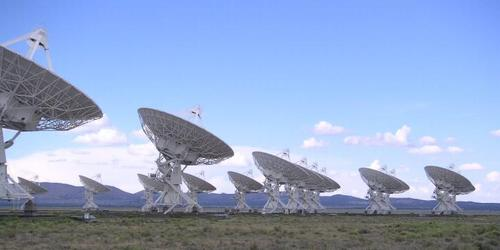
\includegraphics[width=300bp]{USA_NM_VeryLargeArray_03.jpg}

\caption{Arranjo de radiotelescópios - Very Large Array (VLA), New Mexico, EUA. \href{https://commons.wikimedia.org/wiki/File:USA.NM.VeryLargeArray.03.jpg}{Foto: Hajor CC-by-sa}}

\label{est1-fig-9}
\end{figure}


Um arranjo de oito radiotelescópios (A, B, C, D, E, F, G e H) como  ilustrado na \hyperref[est1-fig-9]{Figura \ref{est1-fig-9}} detectou sinais cujos oito registros de tempo para cada radiotelescópio se encontram na tabela a seguir.



\begin{table}[H]
\centering
\begin{tabu} to \linewidth {|c|c|c|c|c|c|c|c|}
\hline
\thead
A & B &  C & D &  E & F &  G &  H \\
\hline
3,03 & 4,37 & 5,04 & 5,73 & 4,03 & 5,37 & 6,04 & 6,74 \\
\hline
3,38 & 4,46 & 5,11 & 5,84 & 4,38 & 5,46 & 6,11 & 6,84 \\
\hline
3,60 & 4,55 & 5,19 & 5,95 & 4,60 & 5,55 & 6,19 & 6,96 \\
\hline
3,78 & 4,63 & 5,29 & 6,08 & 4,78 & 5,64 & 6,29 & 7,08 \\
\hline
3,92 & 4,71 & 5,36 & 6,23 & 4,92 & 5,72 & 6,36 & 7,23 \\
\hline
4,04 & 4,79 & 5,45 & 6,41 & 5,04 & 5,79 & 6,45 & 7,40 \\
\hline
4,16 & 4,87 & 5,54 & 6,62 & 5,16 & 5,87 & 6,54 & 7,63 \\
\hline
4,27 & 4,95 & 5,64 & 6,97 & 5,26 & 5,95 & 6,64 & 7,97 \\
\hline
\end{tabu}
\end{table}

A natureza quantitativa de uma variável contínua pode muitas vezes levar a resultados que praticamente não se repetem. Eles podem ser todos diferentes, como é observado no exemplo. Com o objetivo de identificar alguma estrutura no comportamento deste tipo de variável é necessário agrupar os valores em intervalos de classe, o que permite analisar a sua distribuição de frequências.

\begin{enumerate}
\item Complete a tabela a seguir que utiliza de intervalos de amplitude $0{,}5$ começando em $3{,}0$. Observe que cada intervalo na tabela é fechado à esquerda e aberto à direita, isto quer dizer que, o limite inferior está incluso e o limite superior não está incluso.

\begin{table}[H]
\centering
\begin{tabu} to \linewidth {|c|c|}
\hline
\thead 
Intervalo de classe & Número de observações \\
\hline
${[} 3{,}0 ; 3{,}5 {[}$ & \\ 
\hline
${[} 3{,}5 ; 4{,}0 {[}$ & \\
\hline
${[} 4{,}0 ; 4{,}5 {[}$ & \\
\hline
${[} 4{,}5 ; 5{,}0 {[}$ & \\
\hline
${[} 5{,}0 ; 5{,}5 {[}$ & \\
\hline
${[} 5{,}5 ; 6{,}0 {[}$ & \\
\hline
${[} 6{,}0 ; 6{,}5 {[}$ & \\
\hline
${[} 6{,}5 ; 7{,}0 {[}$ & \\
\hline
${[} 7{,}0 ; 7{,}5 {[}$ & \\
\hline
${[} 7{,}5 ; 8{,}0 {[}$ & \\
\hline
\end{tabu}
\end{table}

Para visualizar o comportamento desses dados, iremos construir um gráfico chamado \index{histograma}histograma, composto por retângulos adjacentes cujas alturas representam a frequência de observações que ocorrem no intervalo correspondente. A base de cada retângulo corresponde aos limites do intervalo definido no agrupamento dos dados.

\item Complete a figura a seguir com os demais retângulos do \hyperref[est1-fig-10]{histograma}.

\begin{figure}[H]
\centering

\begin{tikzpicture} [yscale=0.5, scale=.85]

\foreach \y in {0,...,12}{
   \draw [help lines,color=secundario!50] (-0.1,\y) -- (12,\y);}

\foreach \x in {0,12}{
\draw [help lines, color=secundario!50] (\x,-0.2) -- (\x,12);}

\foreach \x in {1,...,11}{
\draw [help lines, color=secundario!50] (\x,0) -- (\x,-0.2);}

\foreach \y in {0,...,12} \node [left, scale=0.8] at (-0.1,\y) {\y}; 

\foreach \x/\y in {.5/$\leq$ 3.0,1.5/3.0 a 2.5,2.5/3.5 a 4.0,3.5/4.0 a 4.5,4.5/4.5 a 5.0,5.5/5.0 a 5.5, 6.5/ 5.5 a 6.0, 7.5/6.0 a 6.5, 8.5/6.5 a 7.0,9.5/7.0 a 7.5,10.5/7.5 a 8.0,11.5/$>$ 8.0} \node [right, rotate=-90, scale=.8] at (\x, 0) {\y};

\draw [fill=\currentcolor!80] (1,0) rectangle (2,2);
\end{tikzpicture}
\caption{Histograma dos dados coletados pela grade de radiotelescópios}
\label{est1-fig-10}
\end{figure}

\item Calcule a média dos dados da tabela e localize-a no gráfico, sabendo que a soma dos 64 registros de tempo é $351{,}95$. O que você pode observar quanto à localização da média no histograma construído?

\item Calcule a área correspondente ao histograma construído, somando as áreas dos 10 retângulos do histograma. Verifique que o quociente da área de cada retângulo e da área do histograma é igual à frequência relativa do intervalo de classe que ele representa.

\end{enumerate}

\ifdefined\prof
\begin{solucao}
\begin{enumerate}

\item \adjustbox{valign=t}
{
	\begin{tabu} to \linewidth {|c|c|}
	\hline
	\thead 
	Intervalo de classe & Número de observações \\
	\hline
	${[} 3{,}0 ; 3{,}5 {[}$ & 2 \\ 
	\hline
	${[} 3{,}5 ; 4{,}0 {[}$ & 3 \\
	\hline
	${[} 4{,}0 ; 4{,}5 {[}$ & 7 \\
	\hline
	${[} 4{,}5 ; 5{,}0 {[}$ & 9 \\
	\hline
	${[} 5{,}0 ; 5{,}5 {[}$ & 11 \\
	\hline
	${[} 5{,}5 ; 6{,}0 {[}$ & 11 \\
	\hline
	${[} 6{,}0 ; 6{,}5 {[}$ & 9 \\
	\hline
	${[} 6{,}5 ; 7{,}0 {[}$ & 7\\
	\hline
	${[} 7{,}0 ; 7{,}5 {[}$ & 4 \\
	\hline
	${[} 7{,}5 ; 8{,}0 {[}$ & 2 \\
	\hline
	\end{tabu}
}
\clearpage
\item\adjustbox{valign=t}
{
	\begin{tikzpicture} [yscale=0.5, scale=.85]

	\foreach \y in {0,...,12}{
	   \draw [help lines,color=secundario!50] (-0.1,\y) -- (12,\y);}

	\foreach \x in {0,12}{
	\draw [help lines, color=secundario!50] (\x,-0.2) -- (\x,12);}

	\foreach \x in {1,...,11}{
	\draw [help lines, color=secundario!50] (\x,0) -- (\x,-0.2);}

	\foreach \y in {0,...,12} \node [left, scale=0.8] at (-0.1,\y) {\y}; 

	\foreach \x/\y/\z in {.5/0/$\leq$ 3.0,1.5/2/3.0 a 2.5,2.5/3/3.5 a 4.0,3.5/7/4.0 a 4.5,4.5/9/4.5 a 5.0,5.5/11/5.0 a 5.5, 6.5/11/5.5 a 6.0, 7.5/9/6.0 a 6.5, 8.5/7/6.5 a 7.0,9.5/3/7.0 a 7.5,10.5/2/7.5 a 8.0,11.5/0/$>$ 8.0} {\node [right, rotate=-90, scale=0.8] at (\x, 0) {\z};

	\draw [fill=\currentcolor!80] (\x-0.5,0) rectangle (\x+0.5,\y);}

	\node [below, rotate=-0, scale=1, align=center] at (6,-1) {$\bigg\uparrow$ \\ Média};
	\end{tikzpicture}
}

\item A área do histograma construído é dada por $$A=0{,}5\cdot(2+3+7+9+11+11+9+7+3+2)=0{,}5\cdot64=32.$$

Por exemplo, o quociente da área do primeiro retângulo sobre a área total é $$\displaystyle\frac{0{,}5\cdot2}{32}=\frac{13}{2}=264=0,03125$$ que é a frequência relativa desse intervalo de classe. Da mesma forma, o quociente da área do terceiro retângulo sobre a área total é $$\displaystyle\frac{0{,}5⋅\cdot7}{32}=\frac{3{,}5}{32}=\frac{7}{64}=0{,}109375$$ que é a frequência relativa desse intervalo de classe. Essa verificação ilustra a propriedade do histograma em representar a distribuição de frequências dos dados observados tal que cada retângulo do histograma representa a frequência do intervalo de classe correspondente no conjunto de dados como um todo.
\end{enumerate}
\end{solucao}
\fi

\end{document}